\section{Progettazione}\label{chap:progettazione}

La progettazione di un sistema \textit{software} è un'attività che traduce i requisiti in una struttura concreta per 
l'implementazione. Essa coinvolge la definizione dell'architettura, la definizione di \textit{design pattern} e la 
pianificazione delle interazioni tra le componenti del sistema.\\
Il progetto che mi è stato proposto da {\company} ha come obiettivo l'espansione del sistema esistente e non si è reso 
necessario espandere o modificare l'architettura esistente.\\
In questo capitolo descrivo l'architettura di {\movi} che ho studiato al fine di ampliare le funzionalità del sistema.

\subsection{Struttura del \textit{database}}\label{chap:struttura database}

\begin{figure}[H]
    \centering
    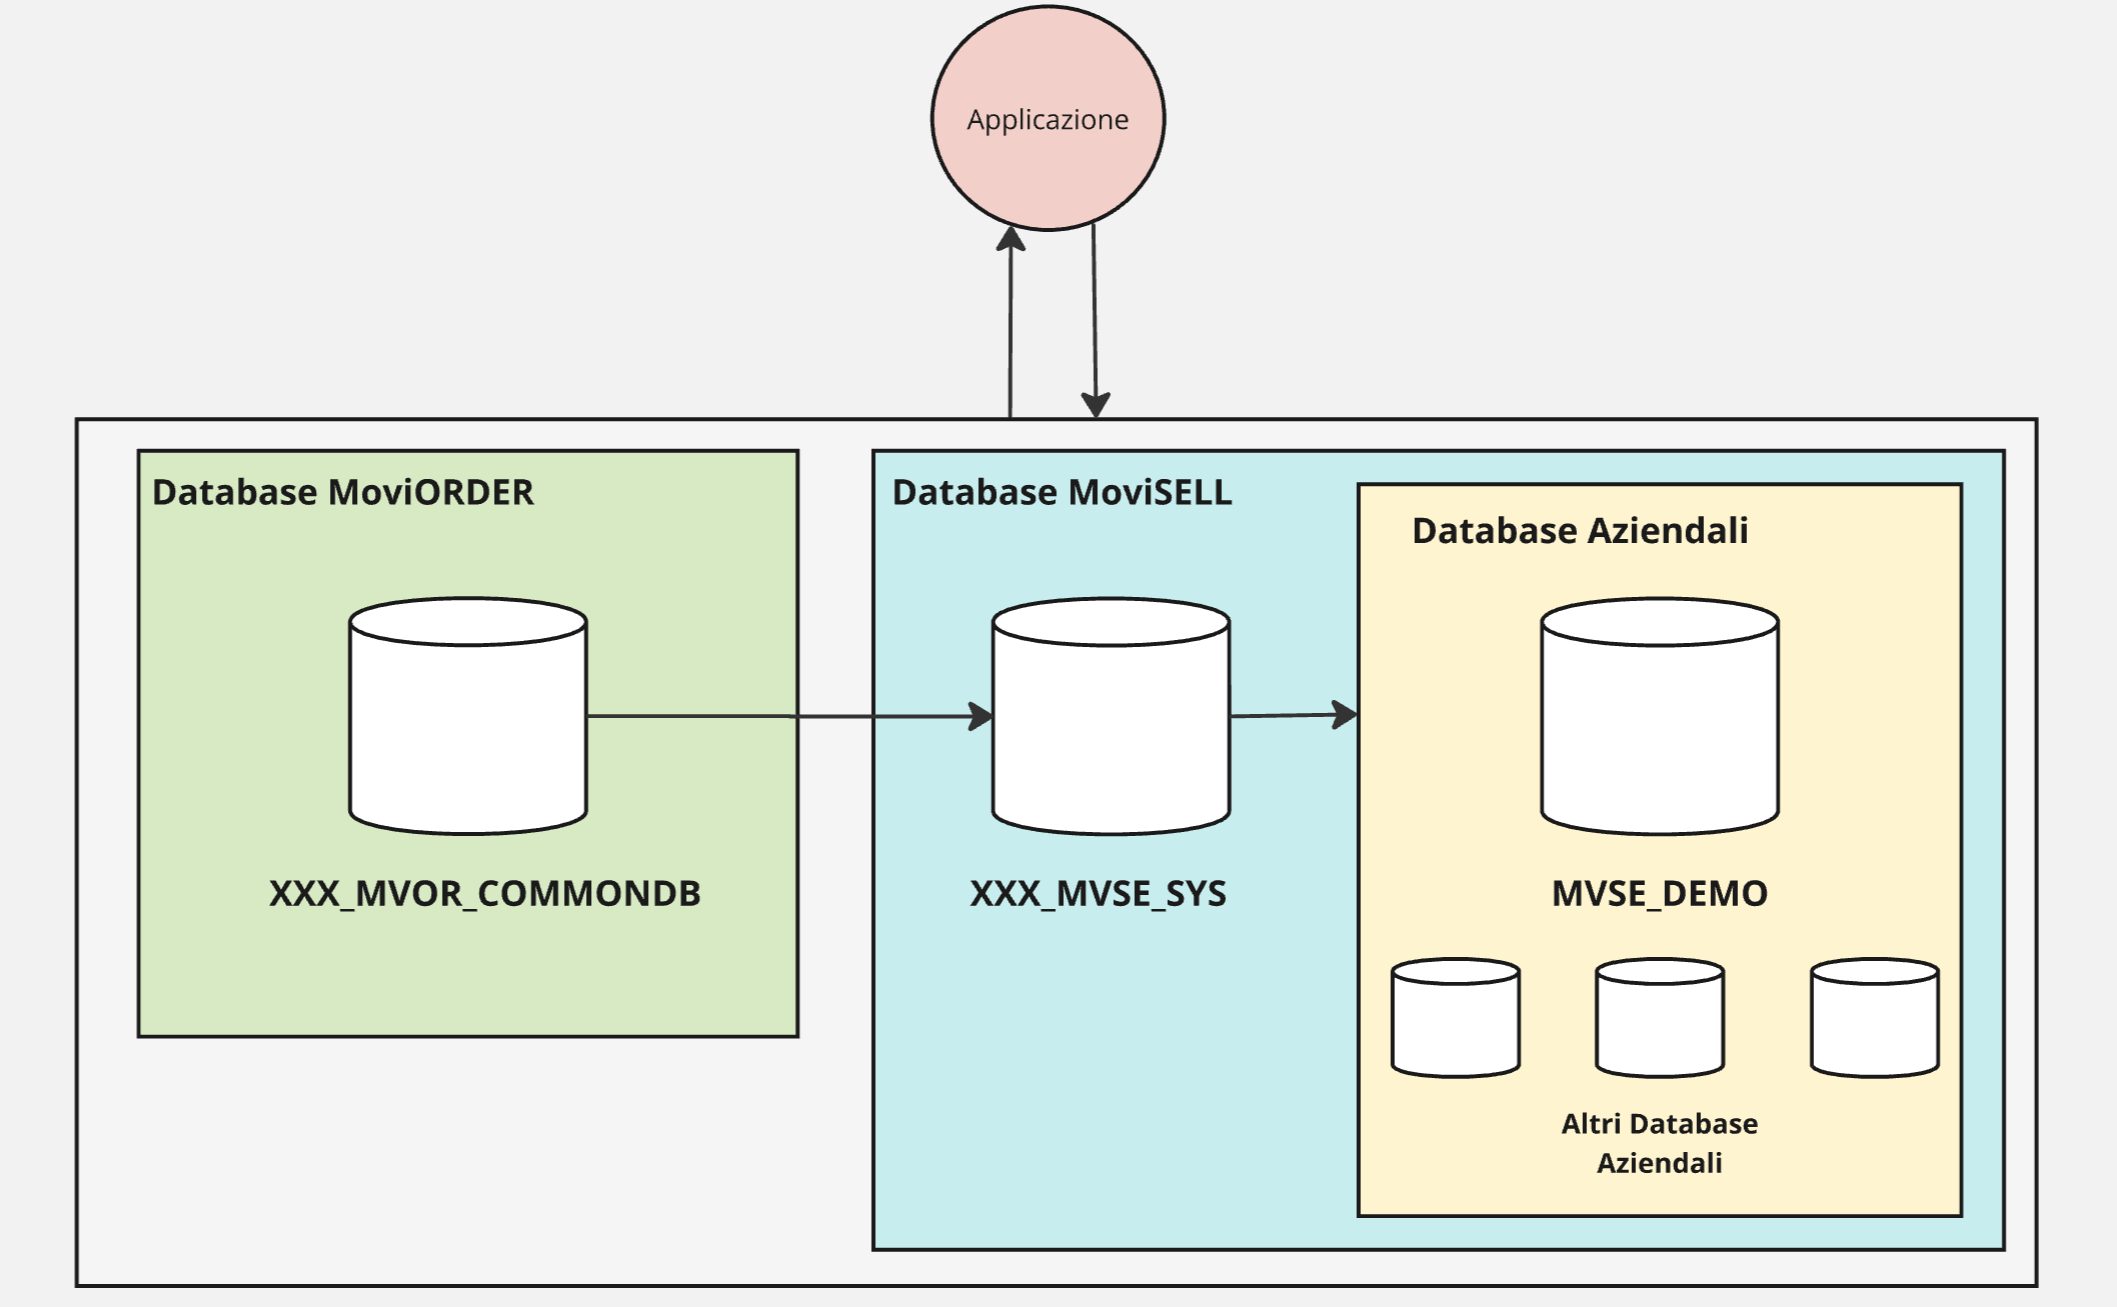
\includegraphics[alt={\textit{Database} di MoviORDER}, width=0.7\textwidth]{img/database.png}
    \caption {\textit{Database} di MoviORDER.}
    \label{fig:database}
\end{figure}

Come illustrato dalla figura \ref{fig:database}, l'infrastruttura dati dell'applicazione {\movi} si articola su tre 
\textit{database} distinti: \texttt{XXX\_MVOR\_COMMONDB}, e i \textit{database} condivisi con l'applicazione 
MoviSELL, ovvero \texttt{XXX\_MVSE\_SYS} e \texttt{MVSE\_DEMO}.\\
\texttt{XXX\_MVOR\_COMMONDB} (che per brevità chiameremo \textit{common database}), contiene i dati relativi a gli utenti di MoviORDER. 
Esso conserva informazioni necessarie all'applicazione come: credenziali di accesso, stato di validità della licenza, 
configurazioni dell'interfaccia utente, dettagli del dispositivo, indirizzi \textit{email} e altri parametri necessari al corretto 
funzionamento del \textit{software}. Questi dati sono fondamentali per i processi di autenticazione e inizializzazione 
dell'applicazione.\\
Ogni azienda ha il proprio \textit{database} dedicato, che chiameremo \textit{company database}, in cui vengono conservati tutti i dati 
a lei inerenti come: anagrafica clienti, catalogo prodotti, politiche di sconto personalizzate, profili degli agenti 
aziendali ecc. Per ogni \textit{company database} viene assegnato un nome del tipo MVSE\_[nome azienda], nel mio caso per lavorare 
in locale mi è stato fornito un \textit{database} di prova chiamato \texttt{MVSE\_DEMO}.\\
Quindi abbiamo \texttt{XXX\_MVSE\_SYS} (che per brevità chiameremo \textit{system database}), il cui scopo è quello di fare da 
\textit{router}, infatti il \textit{common database} contiene un campo nella tabella \texttt{User} chiamato 
\texttt{CompanyCode} che agisce da chiave esterna assegnando ad ogni utente di {\movi} 
un \textit{company database} di riferimento. Questo \texttt{CompanyCode} viene utilizzato dalle \gls{api} come chiave per il 
\textit{system database} per ottenere la stringa di connessione al \textit{company database} durante la fase di autenticazione dell'
utente.\\
Questa architettura garantisce una gestione efficiente e scalabile dei dati, consentendo una separazione netta tra informazioni 
riguardanti l'applicazione e i dati specifici delle aziende, oltre a fornire un meccanismo flessibile per l'indirizzamento 
delle connessioni ai \textit{database} aziendali.
\subsection{Architettura delle API}
Ho continuato quindi il mio studio passando all'analisi dell'architettura delle \gls{api}, che come ho accennato nel capitolo 
\ref{chap:vincoli tec} sono sviluppate utilizzando il \textit{framework} ASP.NET Core. 
Il \textit{back-end} di {\movi} si trova in una \textit{repository} BitBucket a sè stante rispetto al \textit{front-end} per consentire 
una gestione più efficiente e modulare del progetto. Questo permette: 
\begin{itemize}
    \item \textbf{Manutenibilità}: facilita la manutenzione e l'aggiornamento di ciascuna componente senza impattare l'altra;
    \item \textbf{Flessibilità}: permette l'utilizzo di tecnologie e \textit{framework} diversi per \textit{back-end} e 
          \textit{front-end}, ottimizzando ciascuno per il proprio scopo e facilitando eventuali cambiamenti di tecnologie futuri;
    \item \textbf{Versionamento}: consente una versionamento separato per le due parti dell'applicazione e semplifica il 
          tracciamento delle modifiche del codice;
    \item \textbf{Riutilizzo del codice}: Facilita il riutilizzo del \textit{back-end} per diverse interfacce o applicazioni.
\end{itemize}

\begin{figure}[H]
    \centering
    %\hspace{-3.25cm} % Sposta la figura a sinistra di n cm
    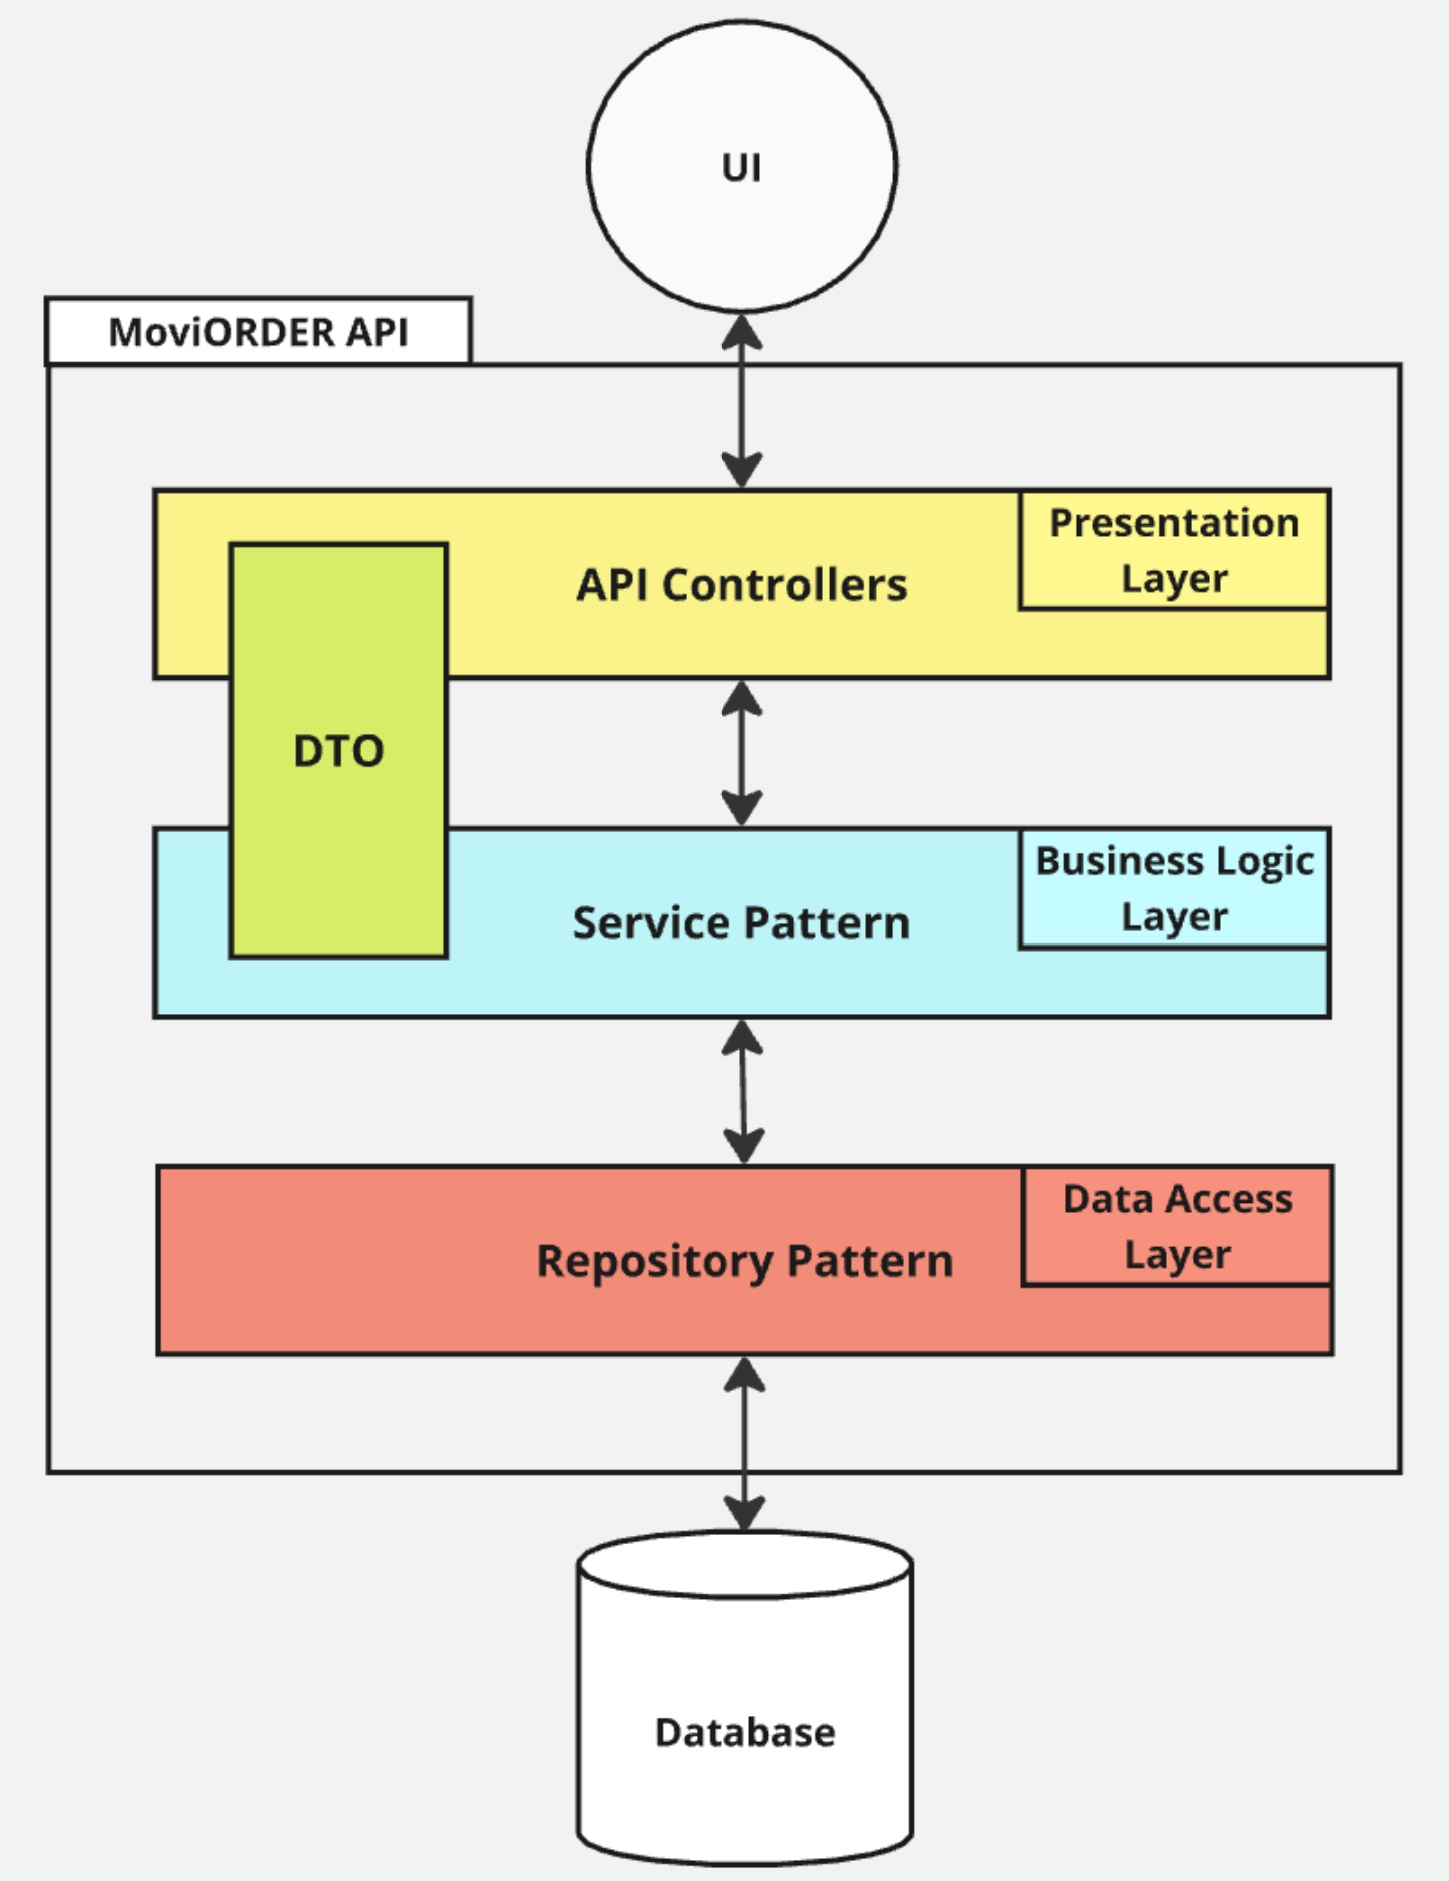
\includegraphics[width=0.6\textwidth]{img/repository-service.jpg}
    \caption{Architettura API.}
    \label{fig:repository-service}
\end{figure}

Le \gls{api} di {\movi} adottano un'architettura a livelli, combinando il \textit{Pattern Repository} e il \textit{Pattern Service}, 
come mostra la figura \ref{fig:repository-service}, garantendo scalabilità, manutenibilità e sicurezza.
Questa architettura stratifica il codice in livelli di astrazione crescente, 
partendo dallo strato più "concreto" in diretta interazione con il \textit{database}, fino a quello più 
"astratto" che si interfaccia con il \textit{front-end}.
\subsubsection{\textit{Data access layer e repository pattern}}
Il \textit{data access layer} di {\movi} è implementato seguendo il \textit{Repository Pattern}, un modello di progettazione 
che separa la logica di accesso ai dati dal resto dell'applicazione. Questo \textit{pattern} crea un'astrazione tra il livello 
di accesso ai dati e la logica di \textit{business}, consentendo una gestione più flessibile e manutenibile dei dati.\\
Il \textit{repository pattern} è implementato attraverso le classi:
\begin{itemize}
\item \texttt{\textbf{ReadOnlyRepository<TContext>}}: Questa classe astratta fornisce metodi per operazioni di sola lettura sul database.
\item \texttt{\textbf{Repository<TContext>}}: Estende \texttt{ReadOnlyRepository} aggiungendo metodi per operazioni di scrittura.
\end{itemize}
Qui vengono definiti anche i modelli e le \textit{migration} generate tramite Entity Framework, un 
\textit{mapper} ad alto livello integrabile a .NET che permette la trasposizione delle tabelle del \textit{database} in 
classi del dominio applicativo.\\
Entity Framework, originariamente parte del \textit{framework} .NET ma ora distribuito come pacchetto indipendente 
installabile attraverso l'\textit{installer} di Visual Studio, promuove un approccio di sviluppo \textit{code first}. 
Entity Framework permette infatti di gestire il \textit{database} attraverso i modelli, ovvero delle particolari classi 
che descrivono la forma delle tabelle e i loro attributi.\\
Creando o modificando questi modelli è possibile creare o modificare la tabella della base dati senza la necessità di 
interventi manuali diretti, ma attraverso le \textit{migration} generate dal \textit{framework} automaticamente. 
Quando si apportano modifiche al modello, Entity Framework compara le \textit{migration} esistenti, determinando così 
lo stato attuale del \textit{database}. Questo processo permette di identificare precisamente le modifiche necessarie 
alla struttura del \textit{database}. Se il processo di analisi e generazione va a buon fine, Entity Framework crea 
una nuova \textit{migration} che riporta tutte le modifiche applicate. Questo meccanismo assicura una gestione 
coerente e tracciabile dell'evoluzione della struttura del \textit{database}, mantenendo sincronizzati il modello dei 
dati nell'applicazione e la struttura effettiva del \textit{database}.\\
In questo caso il \textit{template} \texttt{TContext} delle classi \texttt{Repository} e \texttt{ReadOnlyRepository} 
rappresenta \texttt{DbContext}, una classe fondamentale in Entity Framework che rappresenta una sessione con il 
\textit{database}. Essa permette di:
\begin{itemize}
      \item \textbf{Eseguire query sul database};
      \item \textbf{Tracciare le modifiche apportate alle entità};
      \item \textbf{Persistere i cambiamenti nel database}.
\end{itemize}



\subsubsection{\textit{Business Logic layer e Service Pattern}}

Il \textit{Business Logic layer} in {\movi} implementa il \textit{Service Pattern}, un modello di progettazione 
\textit{software} che separa la logica di \textit{business} dal resto del sistema. Questo \textit{patter} funge 
da intermediario tra il \textit{layer} di presentazione (\textit{API Controllers}) e il \textit{Data Access layer}.\\
Il \textit{Service Pattern} è implementato principalmente attraverso un componente chiave: \texttt{BaseService<TContext, TEntity>} 
che gestisce il flusso di dati, definisce le operazioni CRUD e incapsula la logica dei servizi.\\
I servizi sono classi concrete che estendono \texttt{BaseService} ed implementano la logica di \textit{business} 
che viene richiamata dagli \textit{API Controllers} del livello superiore.\\
Questo approccio offre diversi vantaggi:
\begin{itemize}
\item \textbf{Separazione delle Responsabilità}: la logica di \textit{business} è chiaramente distinta dalla 
      presentazione e dall'accesso ai dati;
\item \textbf{Riusabilità}: le funzionalità incapsulate nei servizi sono facilmente riutilizzabili in diverse 
      parti dell'applicazione;
\item \textbf{Manutenibilità}: la struttura modulare facilita la manutenzione e l'estensione del codice;
\end{itemize}
I servizi gestiscono anche gli errori e mappano i dati in DTO (vedi capitolo \ref{chap:dto}), aumentando la 
modularizzazione.\\
In questo \textit{layer} sono implementati meccanismi di sicurezza basati su \textit{token}. Generato all'autenticazione 
dell'utente, il \textit{token} contiene informazioni criptate utilizzate per verificare identità e permessi ad ogni richiesta 
successiva, garantendo un accesso sicuro alle risorse dell'applicazione.\\
In conclusione, il \textit{Business layer} e il \textit{Service Pattern} in {\movi} forniscono una struttura robusta 
per l'implementazione della logica di \textit{business}, fungendo da ponte efficace tra presentazione e accesso ai 
dati, e assicurando modularità, riusabilità e manutenibilità del codice.
\subsubsection{DTO}\label{chap:dto}
L'utilizzo diretto dei modelli come classi \textit{standard} presenta due criticità:
\begin{itemize}
    \item \textbf{Vulnerabilità nella sicurezza dei dati}: la creazione di istanze dirette dei modelli può esporre 
          involontariamente informazioni sensibili. Un esempio è la tabella \texttt{User} del \textit{common database}, 
          dove tra gli attributi troviamo la \texttt{password} dell'utente. L'utilizzo di queste 
          istanze potrebbe portare alla divulgazione accidentale di dati riservati in parti dell'applicazione dove 
          non sono necessari;
    \item \textbf{Limitazioni nella flessibilità strutturale}: i modelli generati rispecchiano fedelmente la struttura 
        del \textit{database}, ma spesso sono richieste rappresentazioni dei dati più sofisticate o personalizzate. 
          In molti casi, è preferibile definire classi che aggregano o rielaborano dati provenienti da più modelli, 
          offrendo una rappresentazione più adatta alle esigenze funzionali dell'applicazione.
\end{itemize}
Ecco perché vengono introdotti i DTO (\textit{Data Transfer Object}).\\
Essenzialmente, sono contenitori di dati privi di logica di \textit{business}, progettati per trasportare informazioni tra i 
componenti del sistema. Tipicamente contengono solo proprietà pubbliche, senza implementare comportamenti complessi, 
permettendo di controllare precisamente quali dati vengono esposti e trasferiti, migliorando significativamente la 
sicurezza del sistema.\\
Questo è particolarmente importante per proteggere informazioni sensibili, come \textit{password} o altri dati riservati, 
che possono essere omessi o mascherati.\\
L'utilizzo dei DTO incrementa anche la manutenibilità del codice, introducendo un livello di astrazione tra la 
struttura del \textit{database} e la logica applicativa. Questo disaccoppiamento facilita la manutenzione e 
l'evoluzione del codice, permettendo modifiche alla struttura del \textit{database} o alla \textit{Business Logic} 
senza impattare direttamente le interfacce esposte.\\
Quello dei DTO non è un vero e proprio \textit{layer}, ma come mostrato in figura \ref{fig:repository-service} agisce 
da ponte tra il \textit{Presentation layer} e il \textit{Business layer}, in quest'ultimo infatti viene gestita la 
mappatura dei DTO al corrispondente modello in modo da poter convertire un modello in DTO e viceversa.
È possibile anche mappare tra loro i DTO in modo da avere una gestione profonda del passaggio delle informazioni.
\subsubsection{Presentation layer e API controller}
Il \textit{presentation layer} rappresenta lo strato più esterno dell'architettura API di {\movi}, fungendo da interfaccia 
tra il sistema \textit{back-end} e il \textit{front-end}. Questo livello è implementato principalmente attraverso gli 
\textit{API Controller}, che sono responsabili della gestione delle richieste HTTP in ingresso e della formattazione 
delle risposte.\\
Questi \textit{controller} agiscono come punto di ingresso per le richieste \textit{client}, orchestrando il flusso 
di dati e le operazioni tra il \textit{client} e il \textit{business logic layer}.\\
Le principali responsabilità degli \textit{API Controller} includono:
\begin{itemize}
    \item \textbf{Gestione delle richieste}: Ricevono e interpretano le richieste HTTP in arrivo.
    \item \textbf{Routing}: Indirizzano le richieste alle appropriate funzioni del \textit{business logic layer}.
    \item \textbf{Validazione input}: Verificano la correttezza e la sicurezza dei dati in ingresso.
    \item \textbf{Formattazione risposte}: Preparano e inviano risposte HTTP appropriate utilizzando i DTO.
\end{itemize}
Gli \textit{API Controller} interagiscono direttamente con il \textit{business logic layer}, in particolare con i 
servizi che vengono richiamati direttamente nel corpo del \textit{controller}.\\
Tutte le \gls{api} a parte quella per il \textit{login} non possono essere interrogate da un utente non autenticato 
(ovvero che non ha completato la procedura di \textit{login} e che non possiede un \textit{token} valido), in modo 
da concederne l'utilizzo solo a gli utenti di {\movi}.\\
All'interno della cartella dove sono definiti i \textit{controller} troviamo inoltre:
\begin{itemize}
    \item \textbf{\texttt{Program.cs}}: questo file è il punto di ingresso dell'applicazione, dove viene configurato e avviato il 
           \textit{server web} che ospita le \gls{api};
    \item \textbf{Configurazione di Swagger}: ovvero lo strumento usato per il \textit{testing} delle \gls{api};
    \item \textbf{Definizione degli \textit{endpoint}}: ovvero gli indirizzi di connessione ai vari \textit{database} 
          e l'indirizzo in cui le \gls{api} vengono esposte.
\end{itemize}
In conclusione, il \textit{presentation layer} e gli \textit{API Controller} in {\movi} fungono da interfaccia 
tra il mondo esterno e la logica interna dell'applicazione. Attraverso una progettazione attenta e l'uso di DTO, questo 
\textit{layer} garantisce una comunicazione efficiente, sicura e flessibile con il \textit{front-end}, mantenendo al 
contempo una chiara separazione delle responsabilità all'interno dell'architettura complessiva del sistema.
\subsection{\textit{Front-end}}
\subsubsection{\textit{Root} della \textit{repository} e \textit{file} di configurazione}

\begin{figure}[H]
      \centering
      %\hspace{-3.25cm} % Sposta la figura a sinistra di n cm
      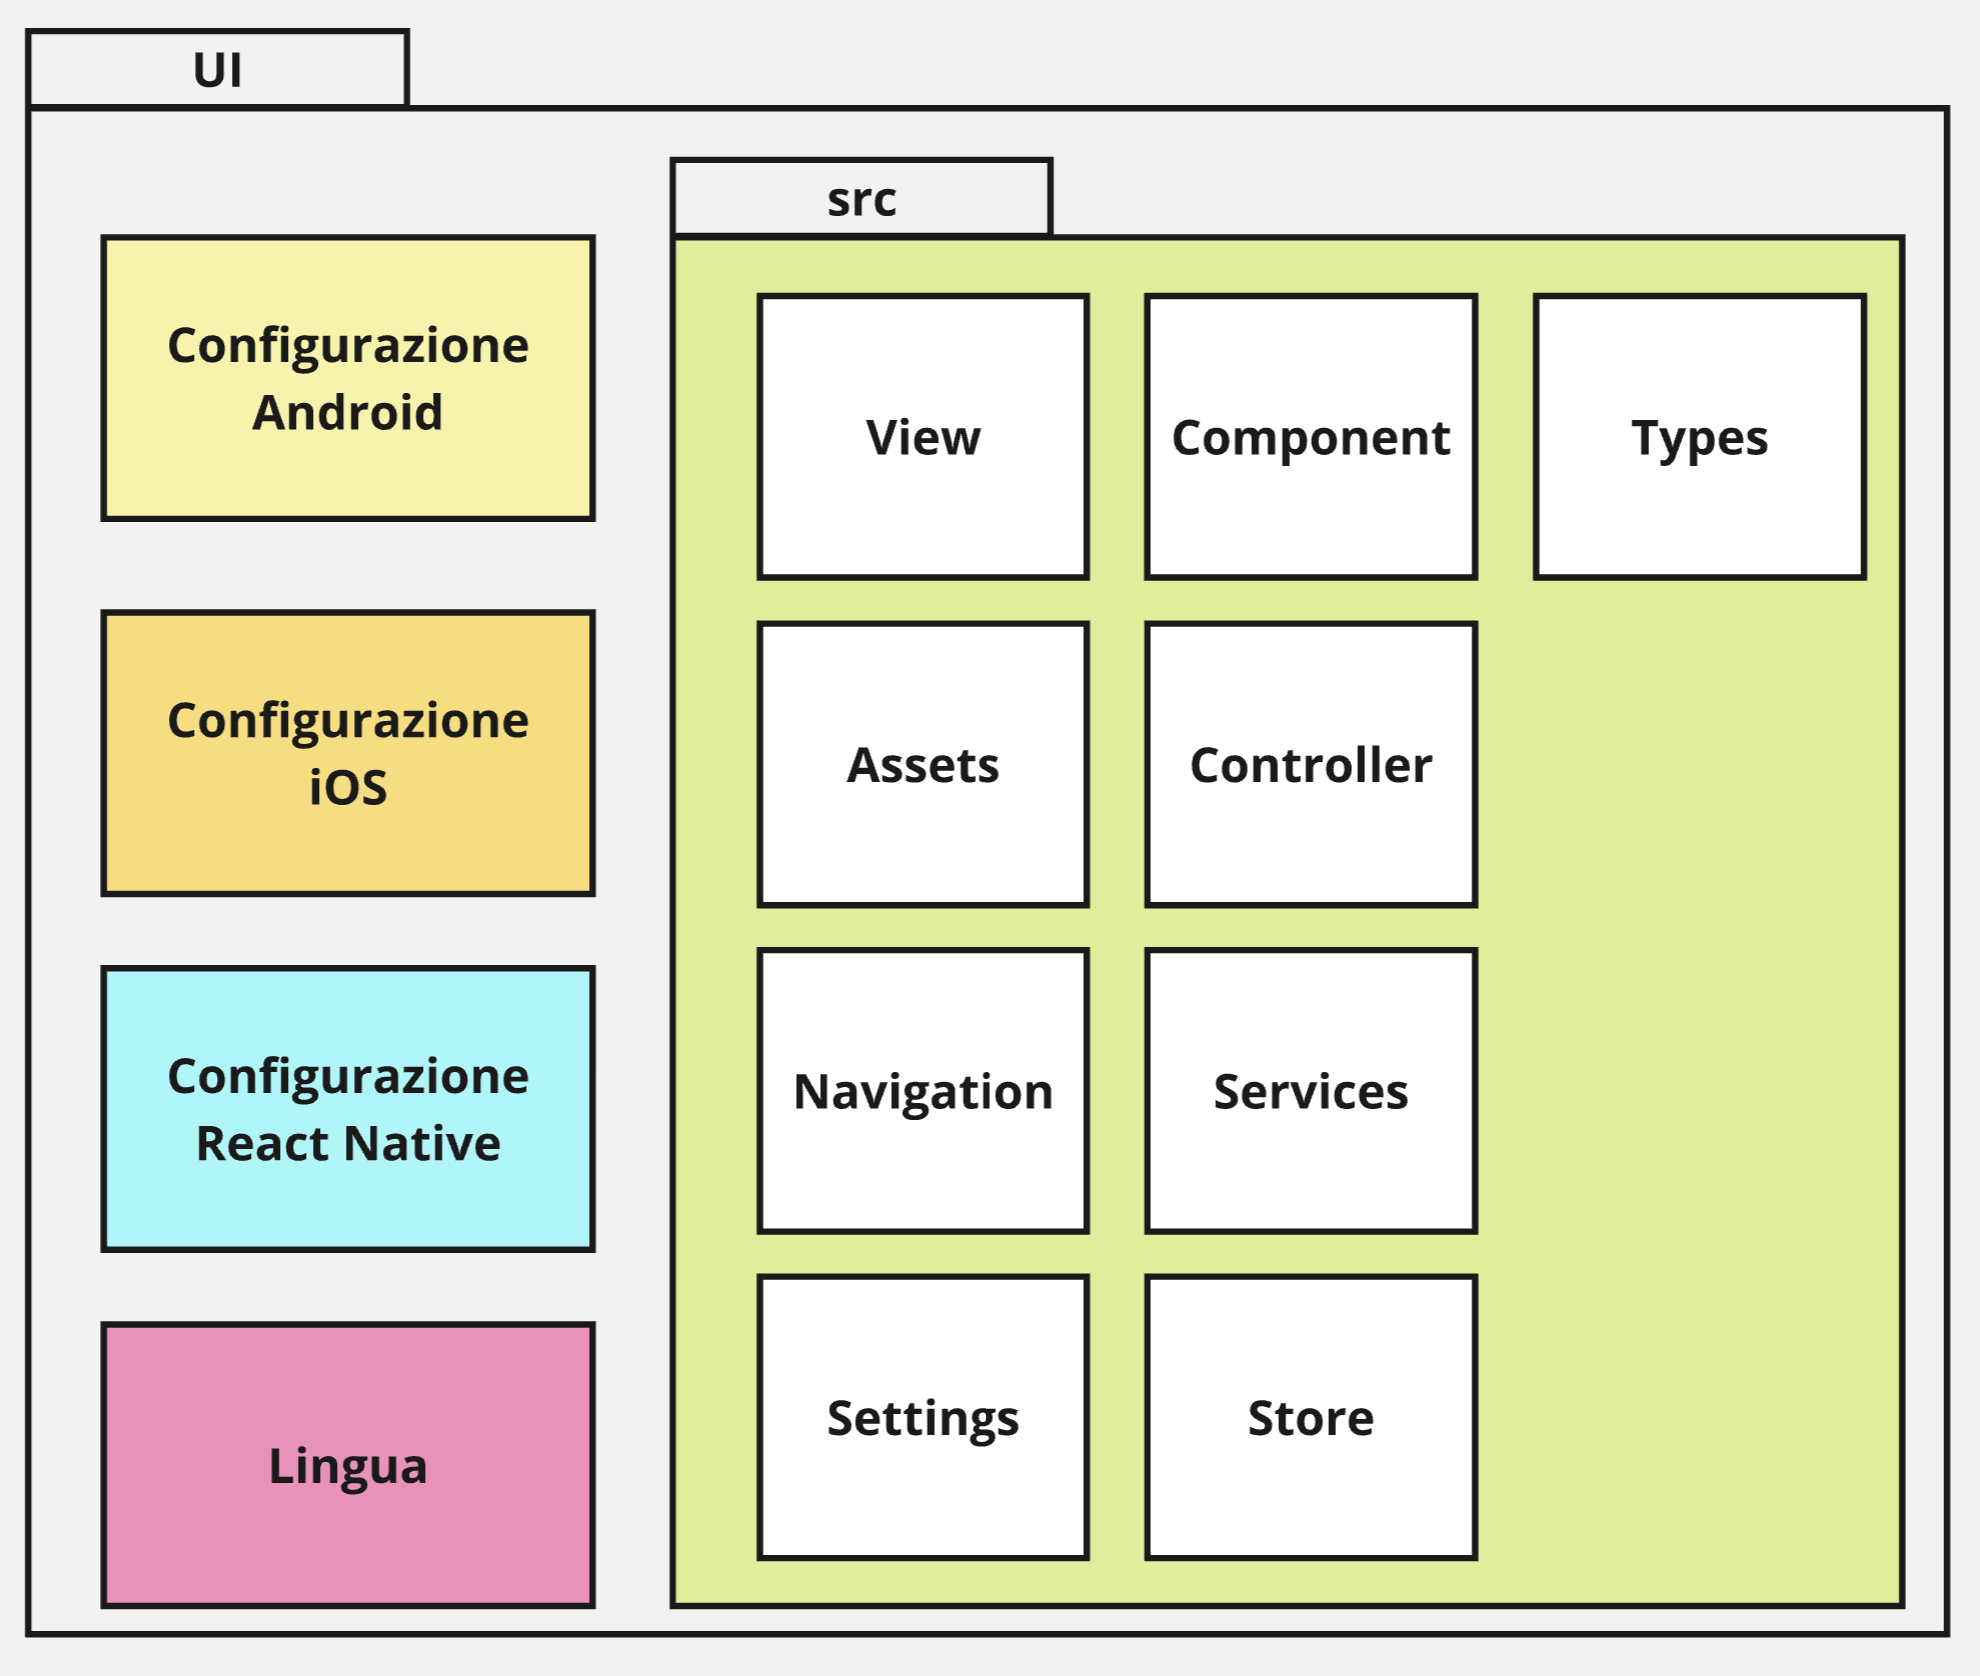
\includegraphics[width=0.6\textwidth]{img/architettura_ui.png}
      \caption{\textit{Root} della \textit{repository} che contiene il \textit{front-end}}
      \label{fig:ui architecture}
\end{figure}

Prima di descrivere l'architettura del \textit{front-end} soffermiamoci ad analizzare il contenuto del \textit{root} della \textit{repository} 
mostrata dalla figura \ref{fig:ui architecture}.
Qui sono contenuti i file di configurazione di React Native e le impostazioni dei compilatori.\\
La \textit{repository} è suddivisa nelle seguenti cartelle:
\begin{itemize}
    \item \texttt{\textbf{Android}}: specifica per React Native, contiene i file di configurazione 
          per la versione Android dell'\textit{app} e \textit{file} come \texttt{build.gradle} e \texttt{AndroidManifest.xml} 
          per la configurazione del compilatore Android;
    \item \texttt{\textbf{iOS}}: specifica per React Native, contiene il progetto Xcode e i file di configurazione 
          per la versione iOS dell'\textit{app} e \textit{file} per la configurazione del compilatore di iOS;
    \item \texttt{\textbf{lang}}: contiene i \textit{file} \texttt{en.json e it.json} che definiscono il testo usato nell'
          applicazione nelle lingue italiano e inglese;
    \item \texttt{\textbf{src}}: contiene tutto il codice del \textit{front-end} e realizza l'architettura;
    \item \textbf{Altri \textit{file} di configurazione}: questi \textit{file} sono fondamentali 
          per garantire un corretto funzionamento e una gestione efficiente del progetto, qui riporto quelli più importanti:
          \begin{itemize}
            \item \textbf{\texttt{package.json}}: contiene le informazioni sul progetto come il nome del progetto, versione,
                  \textit{script} di comando e dipendenze. È il \textit{file} principale per gestire i pacchetti Node.js utilizzati nel progetto;
            \item \textbf{\texttt{yarn.lock}}: questo \textit{file} viene generato automaticamente quando si genera il progetto e 
                  permette di gestire ed installare le dipendenze con le loro versioni esatte;
            \item \textbf{\texttt{metro.config.js}}: configura Metro, il \textit{bundler} di JavaScript predefinito 
                  per React Native. Un \textit{bundler} è uno strumento di sviluppo \textit{software} che combina diversi 
                  \textit{file} di codice sorgente e le loro dipendenze in uno o più \textit{file} ottimizzati, pronti per essere distribuiti 
                  o eseguiti in un ambiente di produzione. Questo \textit{file} permette di personalizzare il comportamento di Metro, come 
                  l'aggiunta di \textit{alias, path} personalizzati, o l'esclusione di determinati \textit{file} dalla \textit{build}.
            \item \textbf{\texttt{babel.config.js}}: configura Babel, il \textit{transpiler} di JavaScript. 
                  Definisce come il codice deve essere trasformato per essere compatibile con le varie versioni di JavaScript e i 
                  diversi ambienti in cui verrà eseguito.
            \item \textbf{\texttt{index.js}}: punto d'ingresso principale dell'applicazione React Native. Qui viene 
                  avviato il \textit{rendering} del componente radice dell'\textit{app};
            \item \textbf{\texttt{app.tsx}}: contiene il componente radice dell'applicazione. Qui vengono definiti l'interfaccia 
                  utente principale e la logica di base dell'\textit{app}.
            \item \textbf{\texttt{tsconfig.json}}: configura il compilatore TypeScript, specificando le opzioni di compilazione 
            e il comportamento del \textit{transpiling} del codice TypeScript in JavaScript.
          \end{itemize}
\end{itemize}
\subsubsection{Architettura React}

\begin{figure}[H]
      \centering
      %\hspace{-3.25cm} % Sposta la figura a sinistra di n cm
      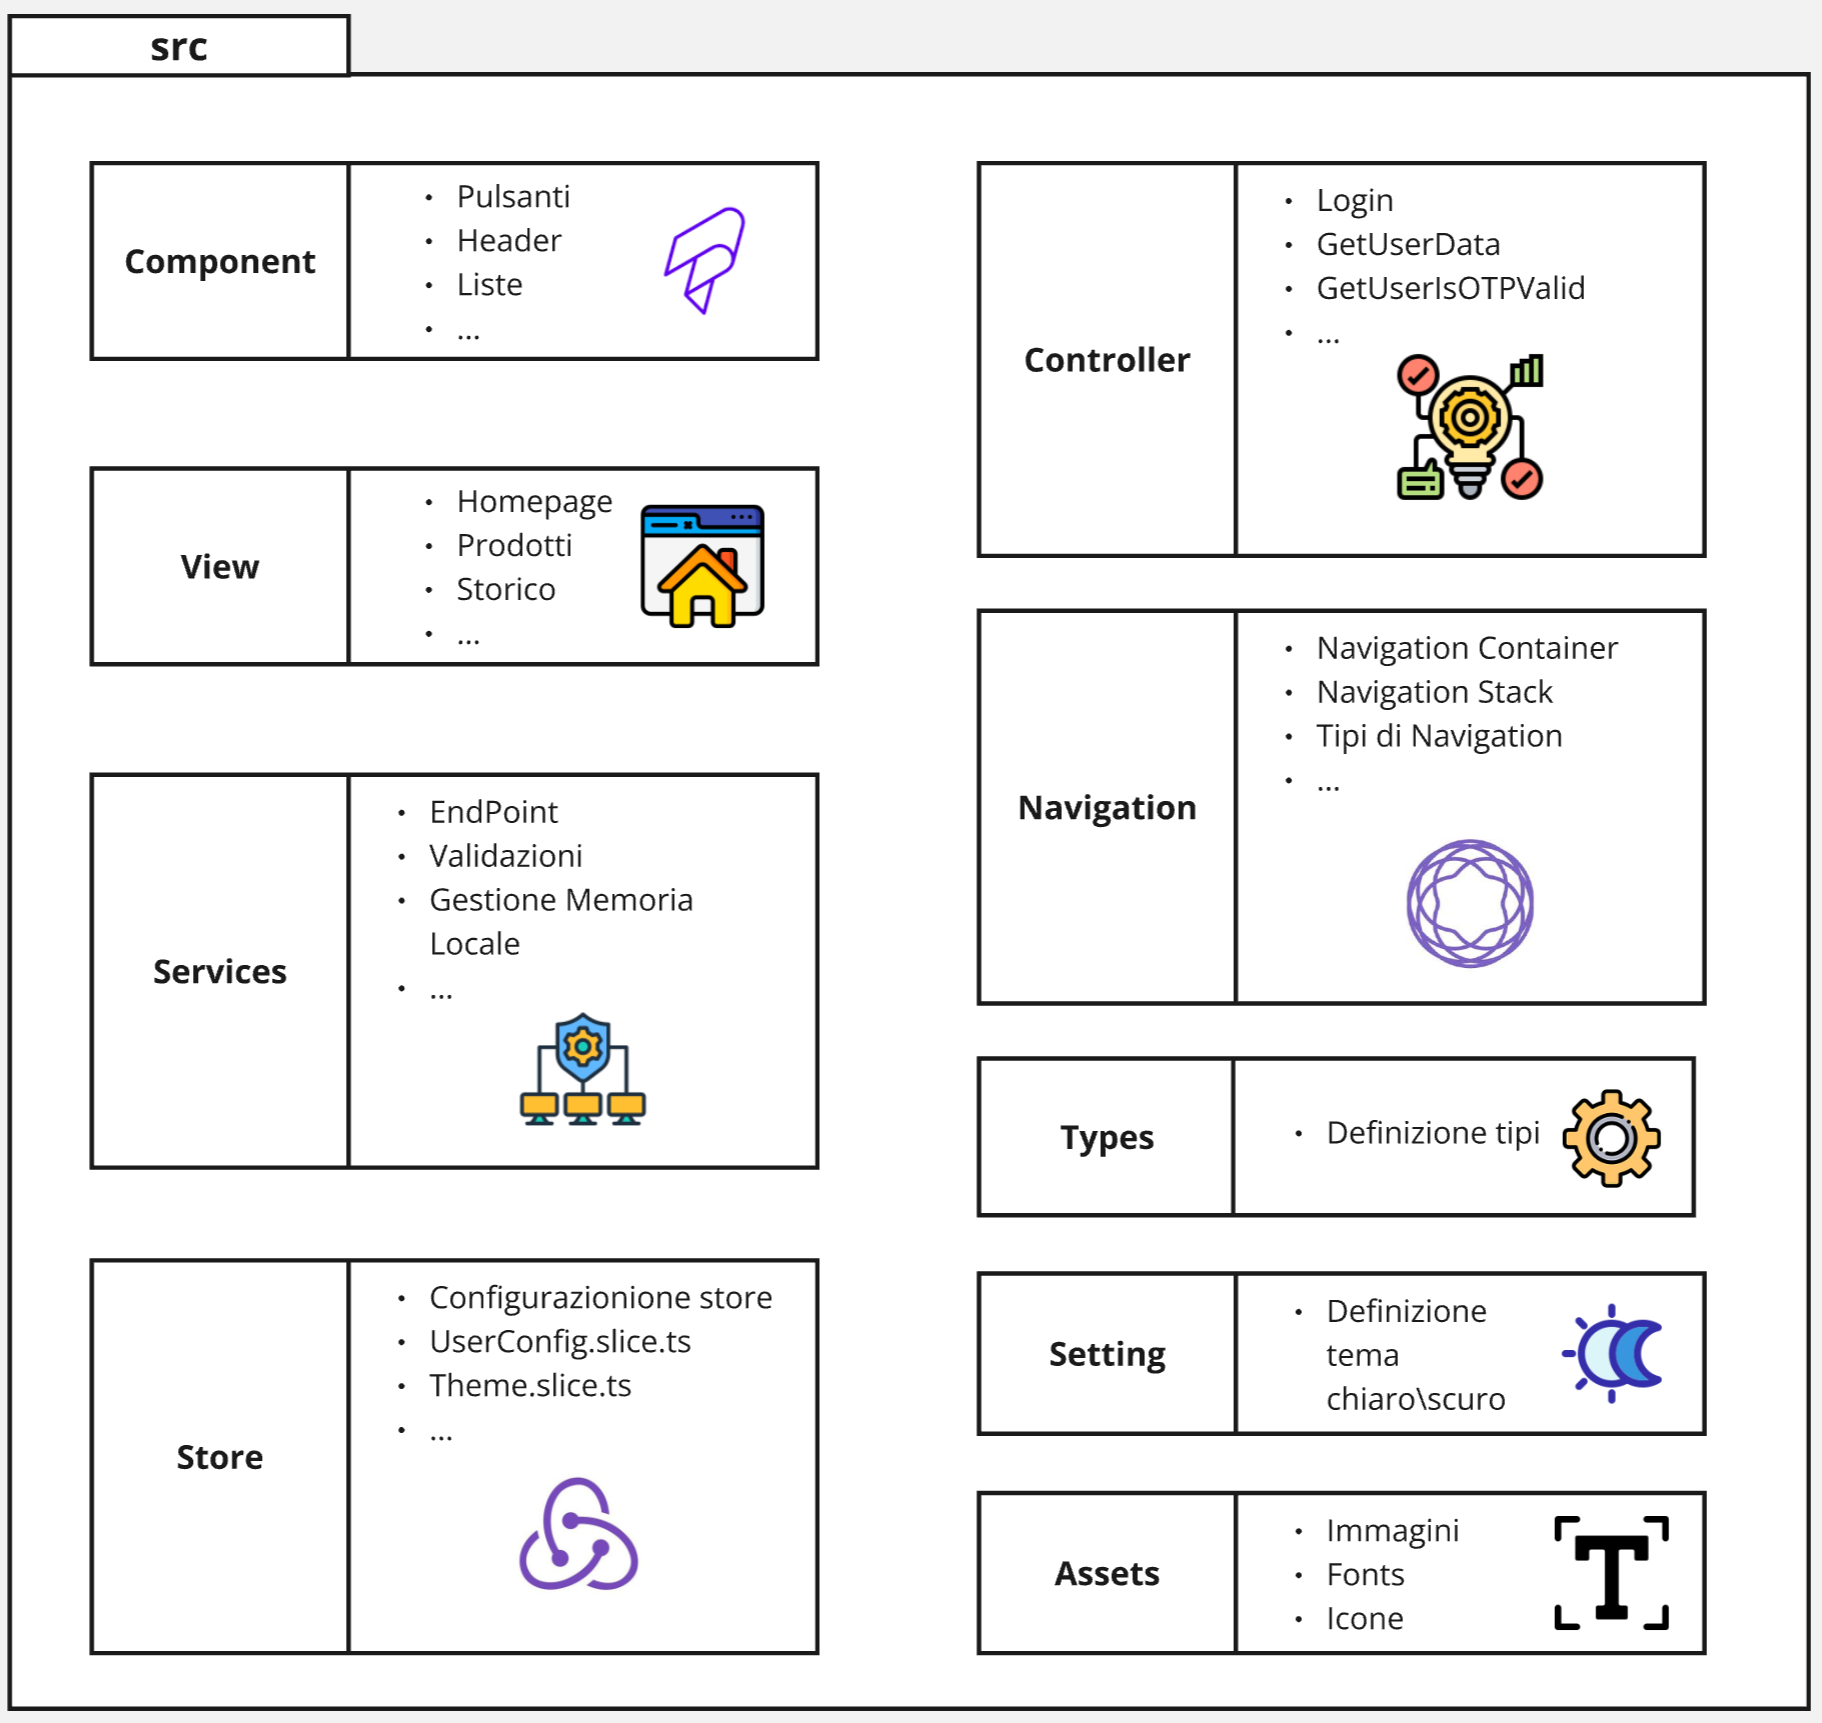
\includegraphics[width=0.8\textwidth]{img/react_architecture.png}
      \caption{Rappresentazione dell'architettura React per {\movi}}
      \label{fig:frontend architecture}
\end{figure}

Una caratteristica distintiva di React è la sua flessibilità nell'implementazione dell'architettura dell'applicazione, 
distinguendosi da altri \textit{framework} JavaScript che impongono modelli predefiniti. Questa libertà consente 
agli sviluppatori di strutturare l'applicazione in base alle specifiche esigenze del progetto.\\
L'architettura React, come illustrata la figura \ref{fig:frontend architecture}, si configura come un insieme di 
componenti responsabili della costruzione dell'interfaccia utente (UI) del \textit{software}. Questa architettura 
può essere concepita come un'organizzazione del codice che facilita la realizzazione di progetti personalizzati, 
includendo vari elementi UI quali pulsanti, moduli, servizi \gls{api} e sistemi di gestione dello stato.\\
L'architettura si articola nelle seguenti directory principali:

\begin{itemize}
      \item \textbf{\texttt{View}}: contiene le pagine complete dell'applicazione, composizioni di 
            componenti più piccoli che formano l'interfaccia utente. Le viste gestiscono la logica e 
            l'organizzazione dei componenti per creare l'esperienza utente complessiva;
      \item \textbf{\texttt{Component}}: ospita componenti UI riutilizzabili e modulari. Questi possono 
            essere elementi come pulsanti, \textit{form}, barre di navigazione o qualsiasi altro elemento 
            dell'interfaccia che può essere utilizzato in più parti dell'applicazione. I componenti in 
            questa cartella sono generalmente più piccoli e più specifici rispetto alle viste;
      \item \textbf{\texttt{Controller}}: contiene la logica di \textit{business} dell'applicazione. Qui 
            si trovano le funzioni e le classi che gestiscono la logica applicativa, elaborano i dati e coordinano le 
            interazioni tra i vari componenti e servizi;
      \item \textbf{\texttt{Services}}: gestisce le interazioni con risorse esterne, come chiamate \gls{api} o la memoria
            del dispositivo. Questa cartella contiene il codice per la comunicazione con il \textit{back-end}, la gestione delle 
            richieste HTTP e l'elaborazione delle risposte. Qui sono definiti inoltre gli \textit{endpoint} per la connessione 
            alle \gls{api};
      \item \textbf{\texttt{Store}}: centralizza la gestione dello stato dell'applicazione utilizzando Redux. Questa cartella 
            contiene la configurazione dello \textit{store} Redux e i \textit{reducer} che definiscono come lo stato dell'applicazione 
            cambia in risposta alle azioni e  dei selettori per accedere allo stato;
      \item \textbf{\texttt{Navigation}}: implementa la logica di \textit{routing} e navigazione dell'applicazione utilizzando 
            React Navigation. Include la mappatura tra i nomi dei \textit{routers} (component che definiscono lo stato della navigazione) 
            e le \textit{view} corrispondenti, nonché opzioni di configurazione per ogni schermata come titoli e animazioni di transizione;
      \item \textbf{\texttt{Types}}: questa cartella contiene le definizioni dei tipi personalizzati utilizzati in tutta l'applicazione. 
            Ciò include interfacce, tipi e enumerazioni che aiutano a mantenere il codice tipizzato e più robusto;
      \item \textbf{\texttt{Assets}}: contiene risorse statiche come immagini, icone, \textit{font} e altri \textit{file} multimediali 
            utilizzati nell'applicazione. Queste risorse sono accessibili e utilizzabili in tutto il progetto;
      \item \textbf{\texttt{Setting}}: definisce i \textit{file} di configurazione per temi (chiaro/scuro).
\end{itemize}